\section{Background}
\label{sec:background}

\begin{figure}[t]
   \centering
   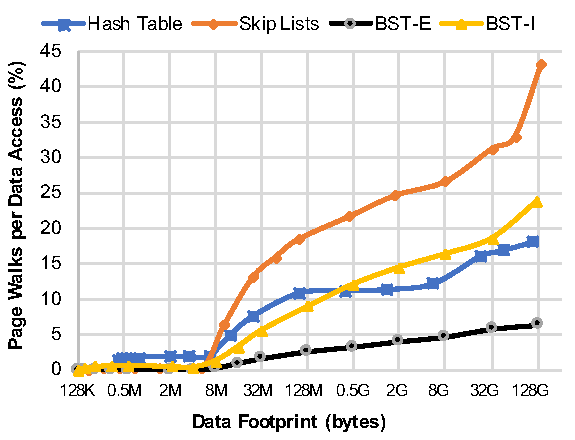
\includegraphics[width=1.0\columnwidth]{graphs/pagewalks.pdf}
   \caption{Frequency of page walks as a function of memory size.}
   \label{fig:pagewalks}
\end{figure}

Today's systems embrace ever increasing mamory sizes, particularly in the server domain where large portions of data are often kept in memory for latency reasons~\cite{}. Such a trend, together with the slowdown in silicon density scaling, forces the system designers to adopt the scale-out approach not only to compute resources, but also to memory resources. This has two major implications on virtual memory: reduced TLB effectiveness and increased page walk latency. 

\subsection{TLB ineffectiveness}
As the memory capacity keeps increasing, TLB hit ratios decrease sharply~\cite{} resulting in significantly higher frequency of page walks. This effect is further exacerbated by increasingly irregular access patterns of modern big data applications that lack spatial and temporal locality~\cite{}. Figure~\ref{fig:pagewalks} shows the number of page walks per memory access as a function of the memory footprint for a set of data traversal benchmarks running on an Intel Broadwell chip (for methodology details, please refer to Section~{sec:methodology}). As expected, the frequency of page walks sharply increases with the size of the data. This result corroborates a prior study on TLB ineffetiveness~\cite{}, which also observed similar trends with larger pages sizes, whose use can only provide one-time reliefs and cannot change the unpromising trend. 

In response, modern systems have embraced larger and more complex TLB hierarchies in an effort to increase the TLB reach. However, increasing the TLB size beyond a few dozen entries provides diminishing returns when accessing hundreds of gigabytes of memory, especially in the absence of spatial and temporal locality~\cite{}. Moreover, the area and power overheads of the TLB hardware become particularly concerning and impractical in heterogeneous systems with a large number of tiny, highly customized accelerators~\cite{}, where the overheads of the translation hardware can greatly surpass the power and area of the rest of the functional parts of the accelerator. Given the increasing gap between the memory growth and practical TLB capacity growth, the TLB performance is certainly not on a promising trajectory.

The underlying reason for poor TLB performance is that TBLs cache translation on the execution side. Because of that, every execution unit (be it a core or accelerator) must have a TLB unit, each of which caches translations that cover the entire physical memory. This is impractical for two reasons. First, the total amount of translation hardware in the system grows linearly with the number of execution units, and second, the memory growth makes each TLB ineffective. In contrast, if we were able to design a system where TLBs would act as memory-side translation caches, each serving one memory partition, then the number of TLBs would not depend on the number of execution units. More importantly, such TLBs would only need to cover a fraction of the dataset, which would significantly increase their TLB hit ratios, as per Figure~\ref{fig:pagewalks}.

\subsubsection{Increasing page walk latency}

As the average distance between compute and memory elements keeps increasing, the latency of page walks, which in the best case (i.e., perfect MMU caches) comprise of one access to a random memory element, increases proportionately.  



\javier{Points to come across:

\begin{itemize}
  \item SW trend: Servers workloads are keeping their datasets memory resident; HW trend: Due to slowdown in silicon density and efficiency, computer system are integrating custom logic (accelerators).
  \item Explain the programmability benefits of pointer-is-a-pointer AND flexible VM system (e.g., demand paging, COW) of a conventional translation mechanism.
  \item TLB Reach Problem: Explain that a conventional translation mechanism is not effective for accelerators because (1) it relies on deep cache and TLB hierarchies and (2) data reuse, to bridge the gap between computation speed and memory capacity. However, accelerators primarily exploit parallel access with proximity to memory, and not reuse and deep cache hierarchies. Furthermore, accelerator are custom and hence silicon optimized, hence the available budget for translation hardware is limited. I think we can just cite prior work on TLB miss rates for in-memory workloads.   
  \item TLB Penalty Problem: Explain that compute and memory are scaling-out due to the slowdown in silicon scaling and efficiency, hence TLB misses (page walks) become more costly. We can show something similar to Figure 1 here.
\end{itemize}


}



